\chapter{Methodology}

\section*{from workplan}
etc

\section{Identification of signal points}
Most of the studies that try to find bathymetric points from Icesat-2 use some variation of the DBSCAN algorithm to identify possible bathymetric signal. The algorithm has the advantages of being robust to noise \cite{} and very computationally efficient. However, one disadvantage is that is is very sensitive to the choice of parameter values, and setting them programatically so that they work on a global scale basis is difficult \cite{} \pdfcomment{does this need better support?}, and many of the previous studies employing this method used a manual review after classification to remove clusters of noise incorrectly labeled as signal \parencite{} \pdfcomment{add citation}. Also, methods based on DBSCAN label points as either likely signal or noise, but then require further interpolation to calculate a sea surface value from the 


\subsection{Filter to subsurface photons}

\pdfcomment{add graphics}
The raw photon cloud from the ATL03 data product contains photons returns from land, clouds, the sea surface, and noise photons. Before applying an algorithm to extract bathymetric signal from noise, first areas of the photon cloud that could not contain bathymetric signal must be removed. A filtering algorithm was developed to cull points in the following order:

\begin{enumerate}
    \item For each point, extract the elevation from the GEBCO dataset. Any points have a GEBCO elevation value of greater than +6m or less than -50m are removed. It is assumed that any points with a GEBCO elevation greater than 6 meters are assumed to be land, and any points with an elevation less than -50 are assumed to be outside the limit of ICESat-2's maximum range for bathymetric sensing (The deepest bathymetric depth found to be detectable by ICESat-2 is 38m. \parencite{Parrish2019})
    
    \item Any points with an elevation greater than 5m above the geoid are assumed to be high noise or land, and are removed from the point dataset.

    \item Calculate the sea surface for each point along the transect. This can be done using the rolling median of the remaining points with window width n=?\pdfcomment{fill in and justify value} of points that are marked as high confidence ocean signal \parencite{Ranndal2021}. Then subtract the Z elevation to get the depth below the ocean surface.  Cull any points deeper than 40m. 
    % This provides the vertical filtering. 
    \item Cull any points within a buffer distance of the sea surface. This removes the strong signal associated with the sea surface.
\end{enumerate}

After applying the filtering steps above, the remaining points are in the area that \emph{could} contain batymetric signal. To determine if there is signal present, further processing is required. There have been several methods for separating bathymetric signal photons from noise, which are explained in section \ref{subsec:denoising}. For this project\pdfcomment{reword?}, a new method is proposed based on a Gaussian Kernel Density Estimation (KDE) function. A function is created that returns the maximum kernel density, and the Z location at which it occurs. Figure \ref{fig:kdefunc} shows the KDE function as applied to two different windows, and the resulting kernel density plots. The KDE function is highly influenced by the \emph{Bandwidth} parameter. For this implementation, the Scott method \citeauthor{Scott2015} is used to estimate the required bandwidth based on the data. 

This function is applied on a rolling basis to a window of 200 points. This function returns a value for every single point along the transect, including in areas that do not have any noticeable signal. The kernel density value gives an indication of the strength of the peak. To reject the locations where the signal is weak, any points with a KDE value of less than $$ kde_{50} - 0.25 * \sigma_{kde} $$ \pdfcomment{maybe just less than median? decreases RMS error}  are assigned an NaN value and are dropped from the analysis.

\begin{enumerate}
    \item apply a window function that finds the kernel density of the subsurface points in the vertical direction. The vertical location of the peak of the kernel density is calculated, as in figure \ref{fig:kdefunc}
    \item If the peak of the kernel density is above a threshold, return the Z elevation of the peak. This is assumed to be the seafloor elevation.
\end{enumerate}

\begin{figure}[htbp]
    \centering
    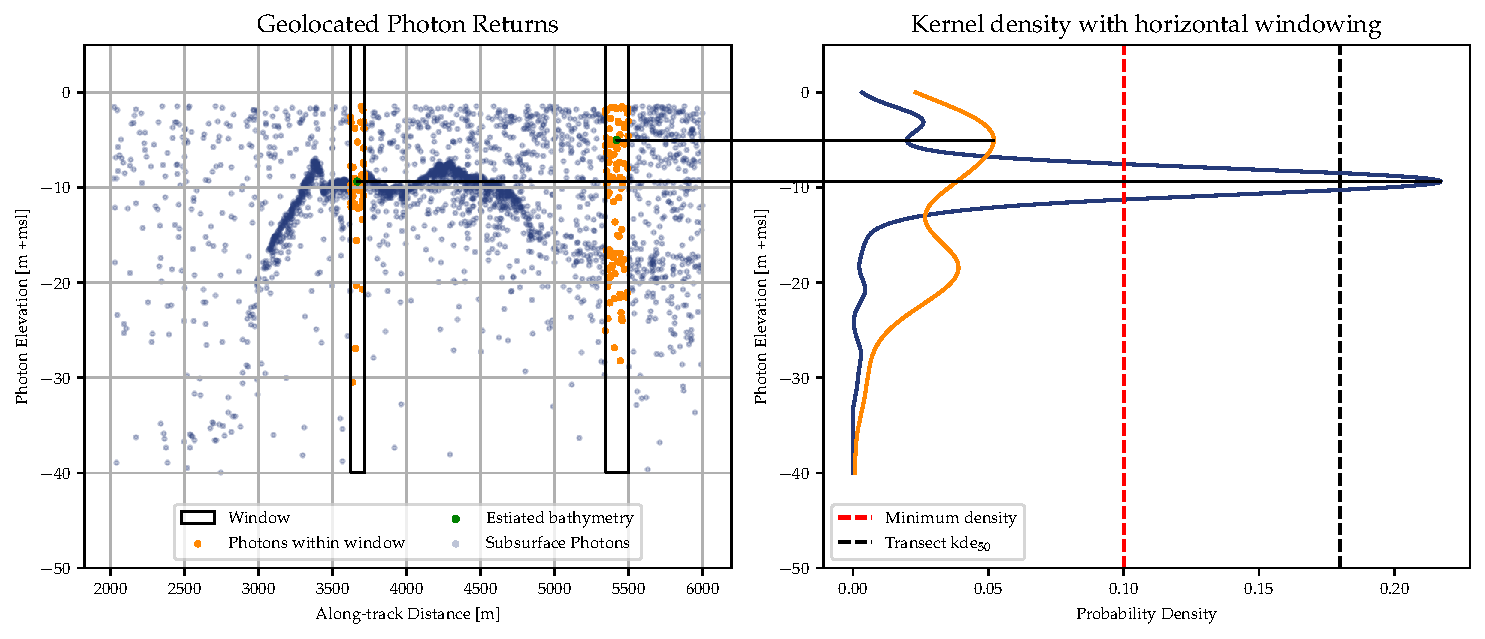
\includegraphics[width=\textwidth]{figures/2d_kde_plot.png}
    \caption{KDE function as applied to 2 different windows}
    \label{fig:kdefunc}
\end{figure}


The input parameters to the signal finding function are:

\begin{enumerate}
    \item The size of the window in \emph{points}
    \item the cutoff value for the Kernel Density required for point to be considered signal
    \item 
\end{enumerate}

\section{Bayesian Data Assimilation using Kalman Filtering}
The Kalman Filter is a mathematical technique to predict the state of systems based on uncertain measurements. It consist of a loop of two steps, an \emph{update} step which updates the position based on a measurement and a known measurement uncertainty, and a \emph{predict} step which predicts the state based on the dynamic equations of the system. 

The Bathymetry of the nearshore zone is assumed to be a static system, and that all measurements are measuring the same system. Since the dynamics are assumed constant, the \emph{predict} step is skipped. To combine multiple measurements, the \emph{update} step can be performed multiple times. 

\subsection*{temp notes}
Instead of using the kalman filter with a state vector of only position, which might just reduce to applying bayes rule recursively, would an MCMC function be a good alternative? 

The kalman filter can indeed by used with only update steps, per wikiepdia: 
\begin{quotation}
    Typically, the two phases alternate, with the prediction advancing the state until the next scheduled observation, and the update incorporating the observation. However, this is not necessary; if an observation is unavailable for some reason, the update may be skipped and multiple prediction procedures performed. Likewise, if multiple independent observations are available at the same time, multiple update procedures may be performed (typically with different observation matrices Hk).[23][24]
\end{quotation}
\begin{itemize}
    \color{orange}
    \item download the xyz data that the gebco data is based on
    \item download and filter photon locations
    \item correct for tide to put them in MSL
    \item Spatially interpolate the resulting XYZ points (Universal kriging?)
    \item Spatially interpolate GEBCO grid (bilinear?)
    \item Run Kalman update step  
\end{itemize}


\section{Selection of Test Sites}
\section{Creation of global analysis sites layer}
\subsubsection*{temp notes}

may 25 - what did I do today:
- rewrote testing notebook to use the updated kde seafloor function, and to include some plots showing the trends in the error (ie. error vs depth, error vs kde value, etc)
- Generated the error for florida, and tried to figure out why it was happening. The error is highly concentrated on a few granules from a certain day - it may be clouds on that day.
- if I look at these transects and see what is going wrong, I might be able to find a way to adapt the algorithm to deal with it.

may 31 -

My current method culls points within a buffer of the sea surface, so it struggles to find signal in very shallow (2-3m) water depth. Maybe A-DRAGANN as implemented in \cite{Cao2021} might be more reliable in shallow water?
\pdfcomment{temp notes}
\begin{enumerate}
    \color{orange}
    \item Start with 2021 OSM coastline
    \item 
    \item clip to extent of mangroves worldwide - only the tropics and subtropics
    \item project in pseudo mercator
    \item split the lines into 100km segments
    \item select these segments where they touch a mangrove 
\end{enumerate}


\section{Processing of Lidar Data}

